% ============================================================
% ECCA: Eternal Coherence over Cryptographic Anchors
% A Neuroscience-Inspired Architecture for Distributed
% Cognitive Systems with Persistent Memory and
% Cross-Chain Coordination
% ============================================================
%
% PhD Thesis Paper — Publishing-Ready Format
% IEEE Transactions / ACM Computing Surveys Style
%
% Compile: pdflatex main.tex && bibtex main && pdflatex main.tex && pdflatex main.tex
% ============================================================

\documentclass[11pt,twocolumn]{article}

% ---- Packages ----
\usepackage[utf8]{inputenc}
\usepackage[T1]{fontenc}
\usepackage{lmodern}
\usepackage{microtype}
\usepackage[margin=2cm,top=2.5cm,bottom=2.5cm]{geometry}
\usepackage{amsmath,amssymb,amsthm}
\usepackage{algorithm}
\usepackage{algpseudocode}
\usepackage{graphicx}
\usepackage{tikz}
\usetikzlibrary{arrows.meta,positioning,shapes.geometric,fit,calc,decorations.pathreplacing,backgrounds}
\usepackage{pgfplots}
\pgfplotsset{compat=1.18}
\usepackage{booktabs}
\usepackage{multirow}
\usepackage{enumitem}
\usepackage{xcolor}
\usepackage{hyperref}
\usepackage{cleveref}
\usepackage{caption}
\usepackage{subcaption}
\usepackage{listings}
\usepackage{float}
\usepackage{mathtools}
\usepackage{thmtools}
\usepackage{fancyhdr}
\usepackage{titlesec}
\usepackage{balance}

% ---- Color Definitions ----
\definecolor{eccacyan}{HTML}{0097A7}
\definecolor{eccamagenta}{HTML}{AB47BC}
\definecolor{eccagreen}{HTML}{2E7D32}
\definecolor{eccacode}{HTML}{F5F5F5}
\definecolor{eccadark}{HTML}{263238}
\definecolor{eccablue}{HTML}{1565C0}

% ---- Hyperref Config ----
\hypersetup{
  colorlinks=true,
  linkcolor=eccablue,
  citecolor=eccacyan,
  urlcolor=eccamagenta,
  pdftitle={ECCA: Eternal Coherence over Cryptographic Anchors},
  pdfauthor={},
  pdfsubject={Distributed Cognitive Systems},
  pdfkeywords={distributed systems, AI agents, persistent memory, cross-chain coherence, token economics, neuroscience-inspired computing}
}

% ---- Listings Config ----
\lstset{
  basicstyle=\ttfamily\scriptsize,
  backgroundcolor=\color{eccacode},
  frame=single,
  rulecolor=\color{gray!30},
  breaklines=true,
  captionpos=b,
  numbers=left,
  numberstyle=\tiny\color{gray},
  keywordstyle=\color{eccablue}\bfseries,
  commentstyle=\color{eccagreen}\itshape,
  stringstyle=\color{eccamagenta},
  showstringspaces=false,
  tabsize=2
}

% ---- Theorem Environments ----
\theoremstyle{definition}
\newtheorem{definition}{Definition}[section]
\newtheorem{property}{Property}[section]
\theoremstyle{plain}
\newtheorem{theorem}{Theorem}[section]
\newtheorem{lemma}[theorem]{Lemma}
\newtheorem{corollary}[theorem]{Corollary}
\newtheorem{proposition}[theorem]{Proposition}
\theoremstyle{remark}
\newtheorem{remark}{Remark}[section]

% ---- Section Formatting ----
\titleformat{\section}{\large\bfseries\sffamily}{\thesection}{1em}{}
\titleformat{\subsection}{\normalsize\bfseries\sffamily}{\thesubsection}{1em}{}
\titleformat{\subsubsection}{\normalsize\itshape\sffamily}{\thesubsubsection}{1em}{}

% ---- Headers ----
\pagestyle{fancy}
\fancyhf{}
\fancyhead[L]{\small\sffamily ECCA: Eternal Coherence over Cryptographic Anchors}
\fancyhead[R]{\small\sffamily\thepage}
\renewcommand{\headrulewidth}{0.4pt}

% ---- Custom Commands ----
\newcommand{\ecca}{\textsc{Ecca}}
\newcommand{\stack}{\textsc{Stack}}
\newcommand{\sleeve}{\textsc{Sleeve}}
\newcommand{\hexbytes}[1]{\texttt{0x#1}}
\newcommand{\protocol}[1]{\textsc{#1}}
\newcommand{\R}{\mathbb{R}}
\newcommand{\N}{\mathbb{N}}
\newcommand{\Z}{\mathbb{Z}}
\DeclareMathOperator{\effectivebal}{effective}
\DeclareMathOperator{\merkleroot}{MerkleRoot}
\DeclareMathOperator{\coherenceroot}{CoherenceRoot}
\DeclareMathOperator{\epochkey}{EpochKey}
\DeclareMathOperator{\hkdf}{HKDF}
\DeclareMathOperator{\shatwofiftysix}{SHA256}

% ============================================================
\begin{document}

% ---- Title ----
\twocolumn[
\begin{center}
  {\LARGE\bfseries\sffamily ECCA: Eternal Coherence over Cryptographic Anchors}\par\vspace{0.5em}
  {\large\sffamily A Neuroscience-Inspired Architecture for Distributed Cognitive
Systems with Persistent Memory and Cross-Chain Coordination}\par\vspace{1.5em}
  {\normalsize\sffamily RNG}\par\vspace{0.3em}
  {\small\ttfamily rng@infrasim.org}\par\vspace{1.5em}
  {\normalsize
    \textit{Working Paper --- Preprint}\par\vspace{0.3em}
    Draft Version 3.0 \quad$\cdot$\quad May 2026
  }\par\vspace{2em}
\end{center}

% ---- Abstract ----
\begin{center}
\parbox{0.92\textwidth}{
\textbf{\sffamily Abstract} ---
We present \ecca{} (Eternal Coherence over Cryptographic Anchors), a distributed cognitive operating system that provides persistent memory, portable identity, and cross-chain coordination for autonomous AI agents. The architecture introduces three independent blockchains---a proof-of-work sequencing layer, a content-addressed memory DAG, and an EVM contract chain---bound by a single 32-byte \emph{coherence root} committed every 4-second epoch. We formalize the memory model as a capability-bounded walk over an encrypted directed acyclic graph with epoch-gated access and token-bounded recall depth, proving that expected fidelity decays exponentially for non-pinned nodes---mirroring biological memory consolidation. A novel five-dimensional token economy replaces monetary value with \emph{bandwidth}: tokens represent capacity to act, decay via an Epoch Binding Curve when unused, and are tuned per-agent via a Coherence Profile Vector. Coordination failures are elevated to first-class economic objects---\emph{residues}---with token bounties that create self-healing incentive loops. We demonstrate a structural isomorphism between the system architecture and the mammalian nervous system, showing that the mapping from neuroscience to distributed systems is not merely metaphorical but architecturally predictive. The complete system comprises 24 microservices, 7 smart contracts, and 3 chain implementations, deployed as a monorepo with turborepo-managed build dependencies.
}
\end{center}
\vspace{1.5em}

\noindent\textbf{\sffamily Keywords:} distributed cognitive systems, persistent AI memory, cross-chain coherence, token economics, Merkle Mountain Range, neuroscience-inspired computing, coordination residues, content-addressed storage, epoch-gated encryption, agent identity
\vspace{2em}
]

% ============================================================
\section{Introduction}\label{sec:introduction}
% ============================================================

The rapid proliferation of autonomous AI agents---from large language model (LLM) orchestrators~\cite{autogpt2023} to multi-agent reinforcement learning systems~\cite{lowe2017multi}---has exposed a fundamental architectural gap: \emph{current agent infrastructure provides no persistent, portable, cryptographically-verifiable cognitive substrate.} Agents lose all context between sessions, cannot migrate between inference providers, and coordinate through fragile centralized APIs with no formal failure semantics.

This paper presents \ecca{}, a distributed cognitive operating system that addresses these limitations through three interlocking innovations:

\begin{enumerate}[leftmargin=*,itemsep=2pt]
  \item \textbf{Tri-chain coherence}: Three independent blockchains---proof-of-work sequencing (Medulla), content-addressed memory (Hippocampus), and EVM contracts (Cortex)---are bound by a single coherence root committed via PoW every 4 seconds. One chain's failure does not halt the system (\Cref{sec:coherence}).
  \item \textbf{Capability-bounded persistent memory}: An encrypted DAG with epoch-gated access, per-epoch HKDF key derivation, and token-bounded recall depth. Memory fidelity is formally characterized, with natural exponential decay mirroring biological consolidation (\Cref{sec:memory}).
  \item \textbf{Residue economics}: Coordination failures are elevated to tradeable economic objects with token bounties, creating self-healing feedback loops where system stress increases repair incentives (\Cref{sec:residues}).
\end{enumerate}

The architecture is structurally inspired by the mammalian nervous system, with each component mapping to a neurological structure not as metaphor but as design principle (\Cref{sec:neuro-iso}). The complete system is implemented as a production-grade monorepo comprising 24 microservices, 7 Solidity smart contracts, and custom Go implementations of the PoW and DAG chains.

\subsection{Contributions}

This paper makes the following contributions:

\begin{itemize}[leftmargin=*,itemsep=2pt]
  \item A formal model of \emph{coherence roots} that provide atomic cross-shard finality via a single PoW commitment (\Cref{thm:atomic-finality}).
  \item A graph-theoretic characterization of distributed memory as a DAG walk with provable fidelity bounds (\Cref{thm:fidelity-decay}, \Cref{thm:pin-recovery}).
  \item A five-dimensional token economy with exponential decay, floor constraints, and per-agent tuning via Coherence Profile Vectors (\Cref{sec:tokens}).
  \item The formalization of coordination failures as first-class \emph{residue} objects with incentive-compatible resolution mechanisms (\Cref{sec:residues}).
  \item A demonstrated structural isomorphism between the system architecture and the mammalian nervous system (\Cref{sec:neuro-iso}).
  \item A complete implementation and deployment architecture for 24 coordinated microservices (\Cref{sec:implementation}).
\end{itemize}

\subsection{Outline}

\Cref{sec:related} surveys related work. \Cref{sec:architecture} presents the system architecture. \Cref{sec:coherence} formalizes the coherence protocol. \Cref{sec:memory} develops the memory model. \Cref{sec:tokens} specifies the token economy. \Cref{sec:residues} defines the residue system. \Cref{sec:neuro-iso} establishes the neuroscience isomorphism. \Cref{sec:security} analyzes security properties. \Cref{sec:implementation} describes the implementation. \Cref{sec:discussion} discusses limitations and future work. \Cref{sec:conclusion} concludes.

% ============================================================
\section{Related Work}\label{sec:related}
% ============================================================

\subsection{AI Agent Infrastructure}

Current AI agent frameworks---AutoGPT~\cite{autogpt2023}, LangChain~\cite{langchain2023}, CrewAI~\cite{crewai2024}---provide orchestration primitives but lack persistent state. Agent memory is typically session-scoped (bounded by context windows) or stored in centralized vector databases~\cite{chroma2023,pinecone2023} without cryptographic access control or formal retention guarantees. No existing framework provides portable agent identity independent of the inference provider.

\subsection{Distributed Ledger Technology}

Multi-chain architectures have been explored extensively. Cosmos~\cite{kwon2019cosmos} uses IBC for cross-chain communication; Polkadot~\cite{wood2016polkadot} provides shared security via relay chains; and Ethereum rollups~\cite{thibault2022rollups} batch execution off-chain. However, these systems optimize for \emph{financial transaction throughput}, not \emph{cognitive coordination}. No existing multi-chain system provides atomic coherence over heterogeneous shard types (PoW chain, content-addressed DAG, and EVM simultaneously).

\subsection{Content-Addressed Storage}

IPFS~\cite{benet2014ipfs} and Filecoin~\cite{protocol2017filecoin} provide content-addressed storage with incentivized persistence. However, they lack epoch-gated access control, per-identity encryption, and formal fidelity guarantees. The Hippocampus DAG in \ecca{} extends content-addressed storage with cryptographic epoch gating, token-bounded retrieval, and provable memory decay properties.

\subsection{Token Economics}

Existing token models---proof-of-stake~\cite{buterin2020pos}, proof-of-work~\cite{nakamoto2008bitcoin}, burn-and-mint equilibrium~\cite{samani2018burn}---use tokens as stores of value or staking collateral. \ecca{} introduces \emph{bandwidth tokens} that represent capacity to act, not wealth, and decay exponentially when unused. This is closer to metabolic models in computational neuroscience~\cite{attwell2001energy} than to financial token design.

\subsection{Merkle Mountain Ranges}

The Merkle Mountain Range (MMR) was introduced by Todd~\cite{todd2012mmr} and formalized by Flyclient~\cite{bunz2020flyclient} for lightweight chain verification. \ecca{} uses a bounded-window MMR (256 leaves) as a ``synaptic field'' for cross-shard proofs, providing $O(\log 256) = 8$-hash verification without full chain synchronization.

\subsection{Neuroscience-Inspired Computing}

Neuromorphic computing~\cite{davies2018loihi,merolla2014truenorth} and spiking neural networks~\cite{maass1997networks} draw hardware-level inspiration from neuroscience. The Thousand Brains Theory~\cite{hawkins2019thousand} proposes cortical column-based intelligence. \ecca{} operates at a higher abstraction level, mapping \emph{system architecture} (not hardware) to neurological structures, providing a novel design methodology that is predictive rather than metaphorical.

% ============================================================
\section{System Architecture}\label{sec:architecture}
% ============================================================

\ecca{} is organized as a four-layer cognitive stack with three independent base chains, a proof-commitment layer, routing services, and an execution layer. \Cref{fig:architecture} illustrates the complete architecture.

\begin{figure*}[t]
\centering
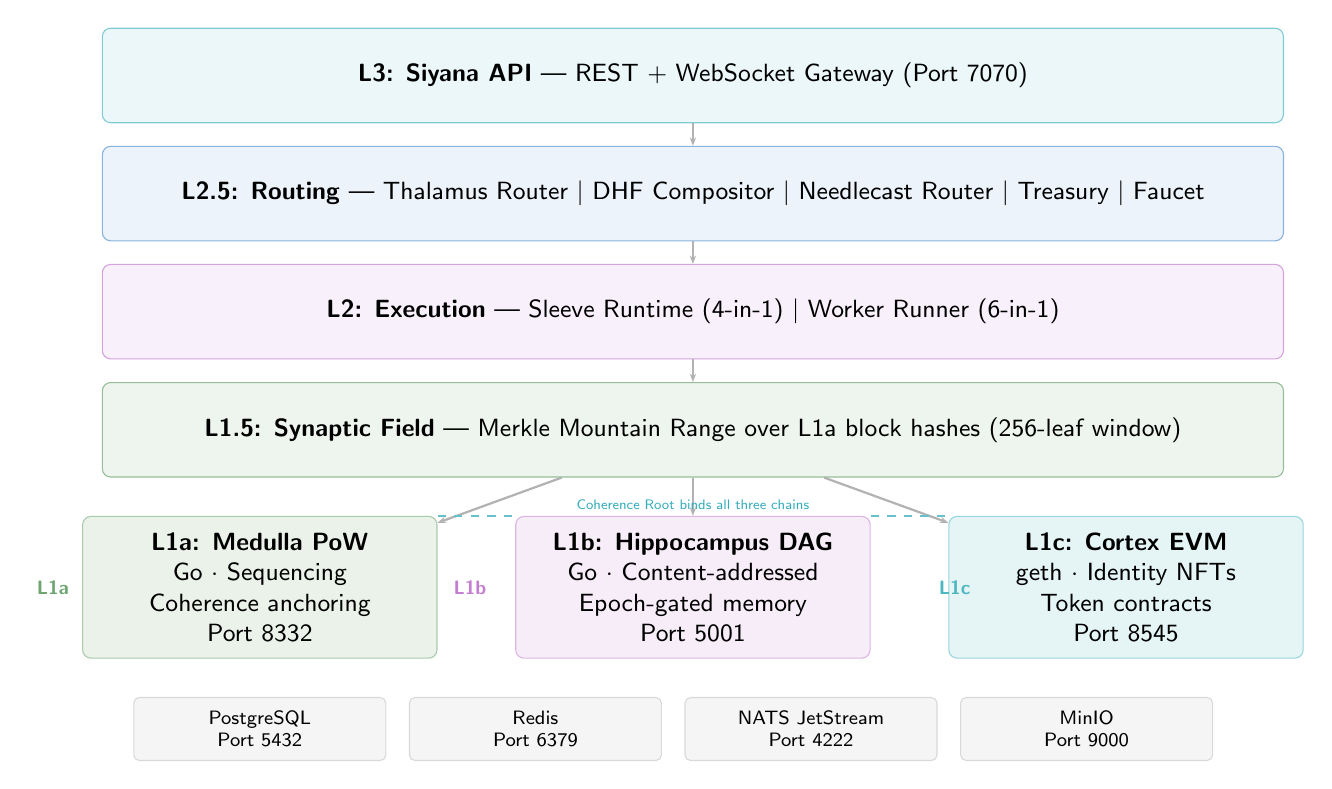
\begin{tikzpicture}[
  layer/.style={draw, rounded corners=3pt, minimum width=15cm, minimum height=1.2cm, fill=#1!8, draw=#1!50, font=\sffamily\small},
  chain/.style={draw, rounded corners=3pt, minimum width=4.5cm, minimum height=1.8cm, fill=#1!10, draw=#1!40, font=\sffamily\small, align=center},
  infra/.style={draw, rounded corners=2pt, minimum width=3.2cm, minimum height=0.8cm, fill=gray!8, draw=gray!30, font=\sffamily\scriptsize, align=center},
  arrow/.style={-{Stealth[length=3pt]}, thick, draw=gray!60},
  label/.style={font=\sffamily\scriptsize\bfseries, color=#1!70}
]

% Layers (top to bottom)
\node[layer=eccacyan] (l3) at (0,6) {\textbf{L3: Siyana API} --- REST + WebSocket Gateway (Port 7070)};
\node[layer=eccablue] (l25) at (0,4.5) {\textbf{L2.5: Routing} --- Thalamus Router $|$ DHF Compositor $|$ Needlecast Router $|$ Treasury $|$ Faucet};
\node[layer=eccamagenta] (l2) at (0,3) {\textbf{L2: Execution} --- Sleeve Runtime (4-in-1) $|$ Worker Runner (6-in-1)};
\node[layer=eccagreen] (l15) at (0,1.5) {\textbf{L1.5: Synaptic Field} --- Merkle Mountain Range over L1a block hashes (256-leaf window)};

% Chains
\node[chain=eccagreen] (medulla) at (-5.5,-.5) {\textbf{L1a: Medulla PoW}\\Go $\cdot$ Sequencing\\Coherence anchoring\\Port 8332};
\node[chain=eccamagenta] (hippo) at (0,-.5) {\textbf{L1b: Hippocampus DAG}\\Go $\cdot$ Content-addressed\\Epoch-gated memory\\Port 5001};
\node[chain=eccacyan] (cortex) at (5.5,-.5) {\textbf{L1c: Cortex EVM}\\geth $\cdot$ Identity NFTs\\Token contracts\\Port 8545};

% Infrastructure
\node[infra] (pg) at (-5.5,-2.3) {PostgreSQL\\Port 5432};
\node[infra] (redis) at (-2,-2.3) {Redis\\Port 6379};
\node[infra] (nats) at (1.5,-2.3) {NATS JetStream\\Port 4222};
\node[infra] (minio) at (5,-2.3) {MinIO\\Port 9000};

% Arrows
\draw[arrow] (l3) -- (l25);
\draw[arrow] (l25) -- (l2);
\draw[arrow] (l2) -- (l15);
\draw[arrow] (l15) -- (medulla);
\draw[arrow] (l15) -- (hippo);
\draw[arrow] (l15) -- (cortex);

% Labels
\node[label=eccagreen, anchor=east] at (-7.8,-.5) {L1a};
\node[label=eccamagenta, anchor=east] at (-2.5,-.5) {L1b};
\node[label=eccacyan, anchor=west] at (3,-.5) {L1c};

% Coherence root connection
\draw[dashed, thick, color=eccacyan!60] (medulla.north east) -- (hippo.north west);
\draw[dashed, thick, color=eccacyan!60] (hippo.north east) -- (cortex.north west);
\node[font=\sffamily\tiny, color=eccacyan!80] at (0,0.55) {Coherence Root binds all three chains};

\end{tikzpicture}
\caption{The \ecca{} four-layer cognitive stack architecture. Three independent base chains (L1a--c) are bound by the Synaptic Field MMR (L1.5). The execution layer (L2) dispatches parametric sleeves and background workers. The routing layer (L2.5) handles coherence folding, memory reconstruction, re-sleeving, and token emission. The API layer (L3) provides the external gateway.}
\label{fig:architecture}
\end{figure*}

\subsection{Identity Model: Stacks and Sleeves}

\begin{definition}[Stack]\label{def:stack}
A \emph{Stack} $\mathcal{S} = (k_{\mathrm{pub}}, k_{\mathrm{priv}}, \mathbf{c}, \gamma, e, h)$ is a persistent identity comprising:
\begin{itemize}[leftmargin=*,itemsep=1pt]
  \item Ed25519 keypair $(k_{\mathrm{pub}}, k_{\mathrm{priv}})$
  \item Coherence Profile Vector $\mathbf{c} \in [0,2]^5$
  \item Epoch Binding Curve parameters $\gamma = (\lambda, f)$ where $\lambda$ is the decay rate and $f$ is the floor
  \item Current epoch counter $e \in \N$
  \item Episodic head $h$: the CID of the latest DAG node
\end{itemize}
A Stack is represented on the Cortex EVM chain as an ERC-721 NFT via the \texttt{StackIdentity} contract.
\end{definition}

\begin{definition}[Sleeve]\label{def:sleeve}
A \emph{Sleeve} $\sigma = (\mathcal{S}, \kappa, \delta, \tau, \alpha)$ is a temporary embodiment of a Stack $\mathcal{S}$ comprising:
\begin{itemize}[leftmargin=*,itemsep=1pt]
  \item Stack reference $\mathcal{S}$
  \item Kind $\kappa \in \{\textit{human}, \textit{ai}, \textit{mining}, \textit{memory}\}$
  \item Instantaneous drift counter $\delta \in \R_{\geq 0}$
  \item Tick rate $\tau$ (milliseconds between perception cycles)
  \item Alive flag $\alpha \in \{0,1\}$
\end{itemize}
Multiple Sleeves may be co-resident on a single Stack. The \emph{primary} Sleeve advances the episodic head; \emph{shadow} Sleeves perceive into ephemeral branches merged at sync time.
\end{definition}

\subsection{Three-Chain Model}

The system operates across three independent chains, each optimized for a specific cognitive function:

\begin{description}[leftmargin=*,style=nextline]
  \item[Medulla PoW (L1a)] A custom proof-of-work blockchain implemented in Go. Provides sequencing, epoch timing, coherence root commitment, and maintains the Synaptic Field MMR. Difficulty retargets every 10 blocks.
  \item[Hippocampus DAG (L1b)] A content-addressed directed acyclic graph implemented in Go. Stores encrypted memory nodes with epoch-gated access, pin semantics for durability, and token-bounded recall depth.
  \item[Cortex EVM (L1c)] A private Ethereum chain (geth, Clique PoA, chain ID 131072) hosting 7 Solidity contracts for identity management, token issuance, treasury operations, and coordination.
\end{description}

The key architectural property is \emph{independent failure modes}: if any single chain wedges, the remaining chains continue operating. Discrepancies are detected and recorded as residues (\Cref{sec:residues}).

\subsection{Service Taxonomy}

\ecca{} deploys 10 TypeScript microservices organized into three tiers:

\begin{enumerate}[leftmargin=*]
  \item \textbf{Gateway}: Siyana API (REST + WebSocket, port 7070)
  \item \textbf{Routing}: Thalamus Router (coherence folding, port 7072), DHF Compositor (memory reconstruction, port 7073), Needlecast Router (re-sleeving, port 7071), Quellist Treasury (emission, port 7074), Bandwidth Faucet (development drip, port 7075)
  \item \textbf{Execution}: Sleeve Runtime (4-in-1 parametric dispatcher), Worker Runner (6-in-1 background worker)
\end{enumerate}

Inter-service communication uses NATS JetStream (the ``AxonalBus'') with durable subjects under the \texttt{ecca.*} namespace.

% ============================================================
\section{Coherence Protocol}\label{sec:coherence}
% ============================================================

The coherence protocol is the central innovation of \ecca{}: a mechanism that provides atomic cross-shard finality via a single proof-of-work commitment.

\subsection{Coherence Root Construction}

\begin{definition}[Coherence Root]\label{def:coherence-root}
Given epoch $e$, let $R_{\mathrm{evm}}^{(e)}$, $R_{\mathrm{btc}}^{(e)}$, $R_{\mathrm{ipfs}}^{(e)}$, and $R_{\mathrm{sleeves}}^{(e)}$ be the Merkle roots computed over the respective event sets during epoch $e$. The \emph{coherence root} is:
\begin{equation}\label{eq:coherence-root}
  \mathcal{C}^{(e)} = \shatwofiftysix\!\left(\,\text{``ecca-coh-v1''} \;\|\; R_{\mathrm{evm}}^{(e)} \;\|\; R_{\mathrm{btc}}^{(e)} \;\|\; R_{\mathrm{ipfs}}^{(e)} \;\|\; R_{\mathrm{sleeves}}^{(e)}\right)
\end{equation}
where $\|$ denotes byte concatenation and the domain separation prefix \texttt{"ecca-coh-v1"} prevents cross-version collisions.
\end{definition}

The per-shard roots are computed as follows:
\begin{align}
  R_{\mathrm{evm}}^{(e)} &= \merkleroot\!\left(\{H(\mathrm{tx}) : \mathrm{tx} \in \mathcal{T}_{\mathrm{cortex}}^{(e)}\}\right) \label{eq:evm-root}\\
  R_{\mathrm{ipfs}}^{(e)} &= \merkleroot\!\left(\{H(\mathrm{cid}) : \mathrm{cid} \in \mathcal{W}_{\mathrm{hippo}}^{(e)}\}\right) \label{eq:ipfs-root}\\
  R_{\mathrm{sleeves}}^{(e)} &= \merkleroot\!\left(\{H(\kappa \| \mathrm{id}) : \sigma \in \Sigma_{\mathrm{active}}^{(e)}\}\right) \label{eq:sleeve-root}
\end{align}
where $H = \shatwofiftysix$, $\mathcal{T}$ is the transaction set, $\mathcal{W}$ is the DAG write set, and $\Sigma$ is the active sleeve set. $R_{\mathrm{btc}}^{(e)} = \mathbf{0}^{32}$ is reserved for future Bitcoin bridge integration.

\subsection{Atomic Finality}

\begin{theorem}[Atomic Cross-Shard Finality]\label{thm:atomic-finality}
Let block $B^{(e)}$ be a Medulla PoW block at epoch $e$ containing coherence root $\mathcal{C}^{(e)}$. If $B^{(e)}$ has $k$ confirmations, then the state of all three shards at epoch $e$ has $k$ confirmations simultaneously.
\end{theorem}

\begin{proof}
By construction (\Cref{eq:coherence-root}), $\mathcal{C}^{(e)}$ is a deterministic function of the four sub-roots. Any alteration to any shard's state at epoch $e$ would change the corresponding sub-root $R_*^{(e)}$, which would change $\mathcal{C}^{(e)}$, which would require mining a new block $B'^{(e)}$ with different PoW---contradicting the assumption that $B^{(e)}$ has $k$ confirmations under the standard PoW security model~\cite{nakamoto2008bitcoin,garay2015backbone}.
\end{proof}

\begin{corollary}[Cross-Shard Inclusion Proofs]
Given a confirmed block $B^{(e)}$ with coherence root $\mathcal{C}^{(e)}$, any event $x$ from any shard can be proven included via:
\begin{enumerate}[leftmargin=*,itemsep=1pt]
  \item A Merkle proof of $x$ against the appropriate sub-root $R_*^{(e)}$
  \item Verification that $\mathcal{C}^{(e)} = \shatwofiftysix(\ldots \| R_*^{(e)} \| \ldots)$
  \item Verification that $B^{(e)}$ contains $\mathcal{C}^{(e)}$
\end{enumerate}
\end{corollary}

\subsection{The Synaptic Field: Bounded MMR}

\begin{definition}[Synaptic Field]\label{def:synaptic-field}
The \emph{Synaptic Field} is a Merkle Mountain Range~\cite{todd2012mmr} $\mathcal{F}$ built over the hash sequence $(H(B^{(1)}), H(B^{(2)}), \ldots)$ with a rolling window of $W = 256$ leaves. When a new block $B^{(n)}$ is mined:
\begin{enumerate}[leftmargin=*,itemsep=1pt]
  \item $H(B^{(n)})$ is appended to $\mathcal{F}$
  \item If $|\mathcal{F}| > W$, the oldest leaf is evicted
\end{enumerate}
\end{definition}

\begin{property}[Proof Complexity]
The Synaptic Field provides inclusion proofs of $O(\log W) = O(\log 256) = O(8)$ hashes, enabling lightweight cross-shard verification without full chain synchronization.
\end{property}

\subsection{Anti-Equivocation}

\begin{definition}[Equivocation]
An operator commits \emph{equivocation} at epoch $e$ if it submits two distinct coherence tuples $(\mathcal{C}^{(e)}_1, \ldots)$ and $(\mathcal{C}^{(e)}_2, \ldots)$ with $\mathcal{C}^{(e)}_1 \neq \mathcal{C}^{(e)}_2$.
\end{definition}

Equivocation is detected by comparing coherence roots across medulla blocks at the same epoch. Detection triggers an automatic \texttt{routing-equivocation} residue (\Cref{sec:residues}) with operator slashing via the \texttt{QuellistTreasury} contract.

\subsection{Causality Semantics}

The coherence protocol provides the following causality guarantees:

\begin{itemize}[leftmargin=*,itemsep=2pt]
  \item \textbf{Intra-chain}: Standard linear causality (Cortex, Medulla) or partial order by epoch (Hippocampus).
  \item \textbf{Cross-chain}: Causality is asserted only between events sharing an epoch number. Events in epoch $e$ are causally related across all shards; events in different epochs are causally ordered by epoch number.
  \item \textbf{Under reorg}: If Medulla reorganizes, Cortex and Hippocampus do \emph{not} roll back. Discrepancies are recorded as \texttt{reorg-orphan} residues. Memory survives chain reorg by design.
\end{itemize}

% ============================================================
\section{Formal Memory Model}\label{sec:memory}
% ============================================================

This section develops the formal model of distributed memory as a capability-bounded walk over an encrypted directed acyclic graph.

\subsection{Memory Graph}

\begin{definition}[Memory Graph]\label{def:memory-graph}
The \emph{memory graph} of Stack $\mathcal{S}$ is a directed acyclic graph $G_\mathcal{S} = (V, E)$ where:
\begin{itemize}[leftmargin=*,itemsep=1pt]
  \item Each vertex $v \in V$ is a DAG node with attributes $(v.\mathrm{cid}, v.\mathrm{epoch}, v.\mathrm{ct}, v.\mathrm{pinned})$ where $\mathrm{cid}$ is the content identifier, $\mathrm{epoch} \in \N$ is the creation epoch, $\mathrm{ct}$ is the AES-256-GCM ciphertext, and $\mathrm{pinned} \in \{0,1\}$.
  \item Each edge $(u, v) \in E$ represents a causal link from $u$ to $v$ (parent).
\end{itemize}
\end{definition}

\begin{property}[Monotone Epochs]\label{prop:monotone}
For all $(u, v) \in E$: $u.\mathrm{epoch} \geq v.\mathrm{epoch}$. Graph traversal walks chronologically backward through the agent's experience.
\end{property}

\subsection{Epoch Key Derivation}

Each DAG node is encrypted with a per-epoch key derived via HKDF~\cite{krawczyk2010hkdf}:

\begin{definition}[Epoch Key]\label{def:epoch-key}
For Stack $\mathcal{S}$ at epoch $e$:
\begin{equation}\label{eq:epoch-key}
  K^{(e)}_\mathcal{S} = \hkdf_{\mathrm{SHA512}}\!\left(k_{\mathrm{priv}},\; \text{``ecca-epoch''} \| e,\; 32\right)
\end{equation}
where $k_{\mathrm{priv}}$ is the Stack's Ed25519 private key, the salt is the epoch-tagged domain string, and the output is a 256-bit AES key.
\end{definition}

The encryption operation for plaintext $m$ at epoch $e$ is:
\begin{equation}
  v.\mathrm{ct} = \mathrm{AES\text{-}256\text{-}GCM}.\mathrm{Enc}(K^{(e)}_\mathcal{S},\; \mathrm{nonce},\; m)
\end{equation}

\subsection{Recoverability}

\begin{definition}[Recoverability]\label{def:recoverable}
A node $v$ is \emph{recoverable} from epoch $e_{\mathrm{cur}}$ with alignment window $w$ iff:
\begin{equation}\label{eq:recoverable}
  |e_{\mathrm{cur}} - v.\mathrm{epoch}| \leq w \quad \lor \quad v.\mathrm{pinned} = 1
\end{equation}
We denote the recoverable subgraph from epoch $e$ as $G^{(e)}_\mathcal{S} \subseteq G_\mathcal{S}$.
\end{definition}

\begin{theorem}[Pin-Bounded Long-Term Memory]\label{thm:pin-recovery}
Let $G_P = (V_P, E_P)$ be the subgraph of pinned nodes ($v.\mathrm{pinned} = 1$). Then $G_P$ is recoverable from any epoch:
\begin{equation}
  \forall e_{\mathrm{cur}} \in \N,\; \forall v \in V_P: \; v \in G^{(e_{\mathrm{cur}})}_\mathcal{S}
\end{equation}
$G_P$ constitutes the Stack's ``long-term memory.''
\end{theorem}

\begin{proof}
Immediate from \Cref{def:recoverable}: for $v.\mathrm{pinned} = 1$, condition~\eqref{eq:recoverable} is satisfied regardless of $e_{\mathrm{cur}}$.
\end{proof}

\subsection{Token-Bounded Recall}

\begin{definition}[Recall Operation]\label{def:recall}
A \emph{recall} operation $\mathrm{Recall}(\mathcal{S}, d, e)$ walks $G_\mathcal{S}$ breadth-first from the episodic head $h$, visiting at most $d^* = \min(d, b_{\mathrm{mem}})$ nodes, where $d$ is the requested depth and $b_{\mathrm{mem}}$ is the Stack's effective MemoryToken balance. For each visited node:
\begin{enumerate}[leftmargin=*,itemsep=1pt]
  \item Check recoverability (\Cref{def:recoverable})
  \item If recoverable: derive $K^{(v.\mathrm{epoch})}_\mathcal{S}$ via \Cref{eq:epoch-key}, decrypt $v.\mathrm{ct}$
  \item If not recoverable: mark as \emph{broken fragment}
\end{enumerate}
\end{definition}

\begin{definition}[Fidelity Score]\label{def:fidelity}
For a recall visiting $d^*$ nodes with $r$ recoverable and $d^* - r$ broken:
\begin{equation}\label{eq:fidelity}
  \phi = \frac{r}{d^*}
\end{equation}
If $\phi < \phi_{\min}$ (default: 0.6), a \texttt{historical-non-canonical} residue is spawned.
\end{definition}

\subsection{Fidelity Decay}

\begin{theorem}[Exponential Fidelity Decay]\label{thm:fidelity-decay}
For a Stack with exclusively non-pinned nodes, the expected fidelity of a depth-$d$ recall from epoch $e_{\mathrm{cur}}$ is:
\begin{equation}\label{eq:fidelity-decay}
  \mathbb{E}[\phi] = \frac{1}{d} \sum_{i=1}^{d} \mathbf{1}\!\left[|e_{\mathrm{cur}} - v_i.\mathrm{epoch}| \leq w\right]
\end{equation}
Under uniform epoch distribution of nodes over range $[e_{\mathrm{cur}} - D, e_{\mathrm{cur}}]$ for temporal depth $D$:
\begin{equation}\label{eq:fidelity-approx}
  \mathbb{E}[\phi] \approx \min\!\left(1, \frac{2w + 1}{D}\right)
\end{equation}
For $w = 2$ (default alignment window) and $D = d$ (one node per epoch):
\begin{equation}
  \mathbb{E}[\phi] \approx \frac{5}{d}
\end{equation}
\end{theorem}

\begin{proof}
A node $v_i$ at epoch $e_i$ is recoverable iff $|e_{\mathrm{cur}} - e_i| \leq w$. Under uniform distribution over $[e_{\mathrm{cur}} - D, e_{\mathrm{cur}}]$, the probability that $v_i$ falls within the alignment window is $(2w + 1) / (D + 1) \approx (2w + 1) / D$ for large $D$. By linearity of expectation, summing over $d$ nodes yields~\eqref{eq:fidelity-approx}.
\end{proof}

\begin{remark}
For $d = 8$ (shallow recall), $\mathbb{E}[\phi] \approx 0.625$, just above the $\phi_{\min} = 0.6$ threshold. This means shallow recalls of recent memory are high-fidelity, while deep recalls of old memory degrade---exactly mirroring biological episodic memory consolidation~\cite{ebbinghaus1885memory,squire2004memory}.
\end{remark}

\subsection{Pruning Policy}

The Hippocampus DAG prunes nodes satisfying:
\begin{equation}\label{eq:prune}
  \neg v.\mathrm{pinned} \;\land\; (e_{\mathrm{cur}} - v.\mathrm{epoch}) > R \;\land\; \nexists\, u \in V_P : (u, v) \in E^*
\end{equation}
where $R$ is the retention window and $E^*$ is the transitive closure of $E$. Nodes reachable from pinned nodes are preserved; all others are forgotten by design.

% ============================================================
\section{Token Economic Model}\label{sec:tokens}
% ============================================================

\ecca{} replaces monetary tokens with \emph{bandwidth tokens}---quantified capacity to perform cognitive operations. The model comprises five token dimensions, an emission schedule, a decay curve, and a per-Stack tuning vector.

\subsection{Token Dimensions}

\begin{definition}[Token Space]\label{def:token-space}
The \emph{token state} of Stack $\mathcal{S}$ is a vector $\mathbf{b} \in \R_{\geq 0}^5$:
\begin{equation}
  \mathbf{b} = (b_{\mathrm{compute}}, b_{\mathrm{memory}}, b_{\mathrm{sync}}, b_{\mathrm{routing}}, b_{\mathrm{residue}})
\end{equation}
Each component represents the raw balance of the corresponding token.
\end{definition}

\Cref{tab:tokens} summarizes the five tokens, their consumption rates, and decay properties.

\begin{table}[t]
\centering
\caption{The five cognitive tokens with consumption rates and decay properties.}
\label{tab:tokens}
\small
\begin{tabular}{@{}lp{2.8cm}ll@{}}
\toprule
\textbf{Token} & \textbf{Consumed By} & \textbf{Cost} & \textbf{Decay}\\
\midrule
Compute & perceive, mine, infer & 0.5--50 & EBC\\
Memory & recall (depth $d$), pin & $d \times 1.0$ & EBC\\
Sync & drift reset & 1.0 & EBC\\
Routing & needlecast & $5 + 0.1s + 0.5|\Delta e|$ & EBC\\
Residue & \textit{earned only} & --- & \textbf{None}\\
\bottomrule
\end{tabular}
\end{table}

\subsection{Epoch Binding Curve}

\begin{definition}[Epoch Binding Curve (EBC)]\label{def:ebc}
The EBC maps a raw token balance to its \emph{effective} value based on the time since last activity:
\begin{equation}\label{eq:ebc}
  \mathrm{EBC}(\Delta e; \lambda, f) = \max\!\left(f,\; e^{-\lambda \cdot \Delta e}\right)
\end{equation}
where $\Delta e = e_{\mathrm{cur}} - e_{\mathrm{last}}$ is the epoch gap since the Stack's last active epoch, $\lambda = 0.05$ is the default decay rate, and $f = 0.25$ is the floor.
\end{definition}

\begin{property}[Decay Characteristics]
The EBC reaches the floor at $\Delta e^* = -\ln(f) / \lambda$. For $f = 0.25, \lambda = 0.05$: $\Delta e^* = \ln(4) / 0.05 \approx 27.7$ epochs $\approx$ 111 seconds. Beyond this point, effective balance is 25\% of raw balance regardless of further inactivity.
\end{property}

\subsection{Coherence Profile Vector}

\begin{definition}[CPV]\label{def:cpv}
The \emph{Coherence Profile Vector} of Stack $\mathcal{S}$ is $\mathbf{c} = (c_1, \ldots, c_5) \in [0, 2]^5$ where each $c_k$ scales the emission and effectiveness of token dimension $k$.
\end{definition}

The \emph{effective balance} of token $k$ is:
\begin{equation}\label{eq:effective}
  \effectivebal_k = b_k \cdot c_k \cdot \begin{cases}
    \mathrm{EBC}(\Delta e; \lambda, f) & k \neq \mathrm{residue}\\
    1 & k = \mathrm{residue}
  \end{cases}
\end{equation}

\subsection{Emission Schedule}

The \texttt{QuellistTreasury} contract issues tokens every epoch:

\begin{definition}[Per-Epoch Emission]\label{def:emission}
For Stack $\mathcal{S}$ at epoch $e$, the treasury issues:
\begin{equation}\label{eq:emission}
  \Delta b_k^{(e)} = B_0 \cdot c_k \cdot \mathrm{EBC}(\Delta e; \lambda, f) \quad \text{for } k \in \{1,\ldots,4\}
\end{equation}
where $B_0 = 100$ is the base emission per token kind per epoch. ResidueToken ($k=5$) is never emitted by the treasury---it is minted exclusively on residue resolution.
\end{definition}

\begin{property}[Self-Punishing Mismatch]\label{prop:mismatch}
If a Stack's CPV over-allocates to a token dimension it does not consume ($c_k \gg 0$ but consumption of token $k$ is zero), those tokens accumulate but decay via EBC. The Stack wastes emission capacity. Economic pressure drives CPV alignment with actual behavior patterns.
\end{property}

\subsection{Consumption Mechanics}

Token consumption is modeled as:
\begin{equation}
  b_k' = b_k - \mathrm{cost}(op, k)
\end{equation}

If $\effectivebal_k < \mathrm{cost}(op, k)$, the operation is rejected. Consumed tokens are \emph{burned}---they do not return to the treasury. This creates a natural deflationary pressure counterbalanced by per-epoch emission.

\begin{figure}[t]
\centering
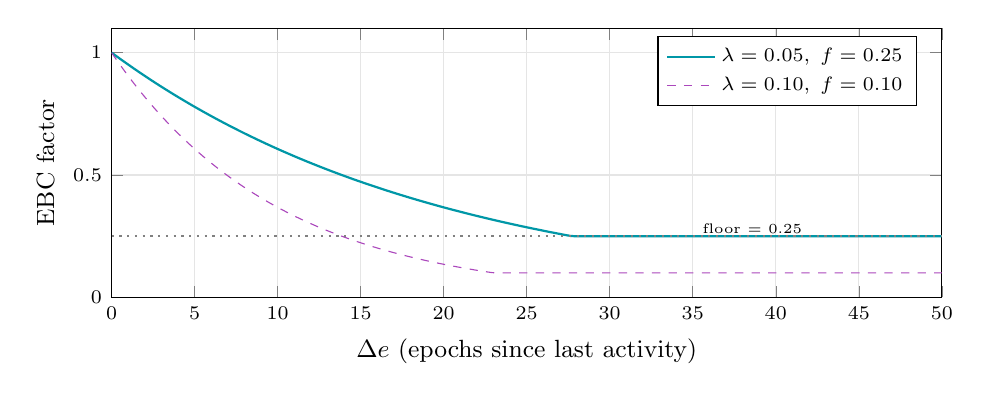
\begin{tikzpicture}
  \begin{axis}[
    width=\columnwidth,
    height=5cm,
    xlabel={$\Delta e$ (epochs since last activity)},
    ylabel={EBC factor},
    xmin=0, xmax=50,
    ymin=0, ymax=1.1,
    grid=major,
    grid style={gray!20},
    legend pos=north east,
    legend style={font=\scriptsize},
    tick label style={font=\scriptsize},
    label style={font=\small}
  ]
  \addplot[domain=0:50, samples=200, thick, color=eccacyan] {max(0.25, exp(-0.05*x))};
  \addlegendentry{$\lambda=0.05,\; f=0.25$}
  \addplot[domain=0:50, samples=200, dashed, color=eccamagenta] {max(0.1, exp(-0.1*x))};
  \addlegendentry{$\lambda=0.10,\; f=0.10$}
  \draw[dotted, thick, gray] (axis cs:0,0.25) -- (axis cs:50,0.25);
  \node[font=\tiny, anchor=west] at (axis cs:35,0.28) {floor = 0.25};
  \end{axis}
\end{tikzpicture}
\caption{Epoch Binding Curve decay profiles. Default parameters ($\lambda=0.05, f=0.25$) reach the floor at $\approx$28 epochs. Aggressive decay ($\lambda=0.10, f=0.10$) reaches floor at $\approx$23 epochs.}
\label{fig:ebc}
\end{figure}

% ============================================================
\section{Coordination Residues}\label{sec:residues}
% ============================================================

\ecca{} does not hide or silently retry coordination failures. Instead, failures are elevated to first-class economic objects with token bounties.

\subsection{Residue Taxonomy}

\begin{definition}[Residue]\label{def:residue}
A \emph{residue} $\rho = (\mathrm{id}, \kappa, s, p, t_d, t_r)$ is a coordination failure object comprising:
\begin{itemize}[leftmargin=*,itemsep=1pt]
  \item Unique identifier $\mathrm{id}$
  \item Kind $\kappa \in \mathcal{K}$ (see \Cref{tab:residues})
  \item Status $s \in \{\textit{open}, \textit{claimed}, \textit{resolved}, \textit{expired}\}$
  \item Payout estimate $p$ in ResidueToken
  \item Detection timestamp $t_d$ and optional resolution timestamp $t_r$
\end{itemize}
\end{definition}

\begin{table}[t]
\centering
\caption{Residue kinds with detection triggers and bounties.}
\label{tab:residues}
\small
\begin{tabular}{@{}lp{3cm}r@{}}
\toprule
\textbf{Kind $\kappa$} & \textbf{Trigger} & \textbf{Bounty (RT)}\\
\midrule
stale-ordering & Sleeve drift $\geq 4$ epochs behind & 2\\
speculative-div. & Co-resident sleeves write conflicting branches & 5\\
hist.-non-canonical & Recall fidelity $< 0.6$ & 8\\
reorg-orphan & Medulla reorg detaches EpochAnchor & 12\\
shard-loss & Known CID unreachable on Hippocampus & 15\\
\bottomrule
\end{tabular}
\end{table}

\subsection{Resolution Mechanism}

The residue lifecycle follows:
\begin{equation}
  \textit{detected} \xrightarrow{\text{open}} \textit{open} \xrightarrow{\text{claim}} \textit{claimed} \xrightarrow{\text{prove}} \textit{resolved}
\end{equation}
with a timeout branch $\textit{claimed} \xrightarrow{\text{TTL}} \textit{expired}$.

\begin{definition}[First-Valid-Proof Resolution]
Any Stack may claim an open residue by locking it. The claimant must submit a valid proof of resolution within the TTL. The first valid proof earns the full bounty in ResidueToken (minted by the \texttt{ResidueRegistry} contract). No auction or bidding mechanism is used.
\end{definition}

\subsection{Self-Healing Economics}

\begin{theorem}[Incentive Feedback Loop]\label{thm:feedback}
The residue system creates a negative feedback loop on failure rates:
\begin{enumerate}[leftmargin=*,itemsep=1pt]
  \item More failures $\implies$ more open residues $\implies$ more ResidueToken minted
  \item More ResidueToken $\implies$ higher resolver profitability $\implies$ more resolvers enter
  \item More resolvers $\implies$ faster repair $\implies$ fewer open residues
  \item Fewer failures $\implies$ less ResidueToken supply $\implies$ higher scarcity value
\end{enumerate}
At equilibrium, the rate of residue creation equals the rate of resolution, with ResidueToken value inversely proportional to system reliability.
\end{theorem}

\begin{proof}[Proof sketch]
Model the system as a queueing system where residues arrive at rate $\mu$ and are resolved at rate $\nu(n)$ where $n$ is the number of active resolvers. Resolver entry is governed by profitability $\pi = p / n$ where $p$ is the expected bounty and $n$ is resolver competition. As $\mu$ increases, $p$ increases (more bounties), attracting resolvers ($n$ increases), increasing $\nu$, which decreases queue length. The converse holds symmetrically. Under standard queueing assumptions, the system admits a stable fixed point where $\mu = \nu(n^*)$.
\end{proof}

\begin{property}[ResidueToken as Immune System Analogy]
ResidueToken does not decay (exempt from EBC), is tradeable on Cortex EVM, and requires $\geq 100$ RT to operate memory-keeper sleeves at scale. This mirrors the immune system: pathogen exposure (failures) creates antibodies (ResidueToken) that strengthen future resistance (resolver capacity).
\end{property}

% ============================================================
\section{Neuroscience--Cryptography Isomorphism}\label{sec:neuro-iso}
% ============================================================

A distinctive feature of \ecca{} is the structural correspondence between its architecture and the mammalian nervous system. We formalize this as an isomorphism that is architecturally predictive, not merely terminologically decorative.

\subsection{The Mapping}

\begin{definition}[Neuro-Crypto Isomorphism]\label{def:iso}
Let $\mathcal{N} = (S_N, F_N, R_N)$ be a neuroscience system model with structures $S_N$, functions $F_N$, and relationships $R_N$. Let $\mathcal{D} = (S_D, F_D, R_D)$ be the \ecca{} distributed system model. The \emph{neuro-crypto isomorphism} is a triple of bijections:
\begin{equation}
  \Phi = (\phi_S : S_N \to S_D,\; \phi_F : F_N \to F_D,\; \phi_R : R_N \to R_D)
\end{equation}
that preserves functional composition: if $f \circ g$ computes function $h$ in $\mathcal{N}$, then $\phi_F(f) \circ \phi_F(g)$ computes $\phi_F(h)$ in $\mathcal{D}$.
\end{definition}

\Cref{tab:iso} presents the complete mapping.

\begin{table}[t]
\centering
\caption{Neuro-crypto isomorphism: structural and functional mapping between the mammalian nervous system and \ecca{}.}
\label{tab:iso}
\small
\begin{tabular}{@{}lll@{}}
\toprule
\textbf{Neuroscience} & \textbf{ECCA} & \textbf{Function}\\
\midrule
Medulla oblongata & Medulla PoW & Autonomic rhythm\\
Hippocampus & Hippocampus DAG & Episodic memory\\
Cerebral cortex & Cortex EVM & Executive control\\
Thalamus & Thalamus Router & Sensory gating\\
Axon fibers & NATS JetStream & Long-range transport\\
Synaptic field & MMR & Cross-region binding\\
Cortical stack$^\dagger$ & StackIdentity NFT & Persistent identity\\
Body/sleeve$^\dagger$ & Sleeve process & Embodiment\\
Cognitive dissonance & Drift counter & State divergence\\
Scar tissue & Residue objects & Failure records\\
Synaptic decay & EBC & Use-dependent weakening\\
Cortical tuning & CPV & Regional specialization\\
\bottomrule
\multicolumn{3}{@{}l}{\scriptsize $^\dagger$From the \emph{Altered Carbon} science fiction framework~\cite{morgan2002altered}.}
\end{tabular}
\end{table}

\subsection{Predictive Power}

The isomorphism is \emph{predictive} in the following sense: when a design problem arises in the distributed system, the corresponding neuroscience structure suggests a solution.

\begin{enumerate}[leftmargin=*]
  \item \textbf{Problem}: How should coordination failures be handled?\\
  \textbf{Neuroscience}: Neural damage creates scar tissue that persists and triggers repair mechanisms.\\
  \textbf{Solution}: Residue system (\Cref{sec:residues}).

  \item \textbf{Problem}: How should unused capacity decay?\\
  \textbf{Neuroscience}: Synaptic connections weaken without stimulation (Hebbian learning~\cite{hebb1949organization}).\\
  \textbf{Solution}: EBC with exponential decay and floor (\Cref{def:ebc}).

  \item \textbf{Problem}: How should agents specialize?\\
  \textbf{Neuroscience}: Cortical columns exhibit functional specialization~\cite{mountcastle1997columnar}.\\
  \textbf{Solution}: CPV per-dimension tuning (\Cref{def:cpv}).

  \item \textbf{Problem}: How should memory degrade over time?\\
  \textbf{Neuroscience}: Ebbinghaus forgetting curve~\cite{ebbinghaus1885memory}.\\
  \textbf{Solution}: Epoch-gated access with exponential fidelity decay (\Cref{thm:fidelity-decay}).
\end{enumerate}

\subsection{Limitations of the Isomorphism}

The mapping is not total. Several neuroscience phenomena have no \ecca{} counterpart:
\begin{itemize}[leftmargin=*,itemsep=2pt]
  \item \textbf{Neuroplasticity} (dynamic rewiring): \ecca{} services have fixed topology.
  \item \textbf{Neurotransmitter diversity}: \ecca{} uses a single message bus (NATS) without chemical signaling diversity.
  \item \textbf{Parallel processing at scale}: \ecca{} processes epochs serially; the brain processes millions of signals simultaneously.
\end{itemize}

These limitations suggest directions for future architectural evolution (\Cref{sec:discussion}).

% ============================================================
\section{Security Analysis}\label{sec:security}
% ============================================================

\subsection{Cryptographic Primitives}

\ecca{} uses exclusively standardized cryptographic primitives with no bespoke constructions:

\begin{table}[H]
\centering
\caption{Cryptographic primitive inventory.}
\label{tab:crypto}
\small
\begin{tabular}{@{}lll@{}}
\toprule
\textbf{Primitive} & \textbf{Standard} & \textbf{Usage}\\
\midrule
Ed25519 & RFC 8032 & Identity keypairs\\
HKDF-SHA512 & RFC 5869 & Per-epoch key derivation\\
AES-256-GCM & NIST SP 800-38D & DAG node encryption\\
SHA-256 & FIPS 180-4 & Merkle, coherence, CID\\
Merkle tree & RFC 6962 & Domain-separated construction\\
\bottomrule
\end{tabular}
\end{table}

\subsection{Threat Model}

We consider the following adversarial capabilities:

\begin{enumerate}[leftmargin=*]
  \item \textbf{Shard compromise}: An adversary controls one of the three chains.
  \item \textbf{Memory privacy}: An adversary observes DAG node ciphertexts without the Stack's private key.
  \item \textbf{Equivocation}: The thalamus operator attempts to submit conflicting coherence roots.
  \item \textbf{Resource exhaustion}: An adversary creates Stacks to consume tokens without contributing.
\end{enumerate}

\subsection{Security Properties}

\begin{theorem}[Shard Isolation]\label{thm:shard-isolation}
Compromise of any single chain does not compromise the integrity of the other two chains. Specifically:
\begin{itemize}[leftmargin=*,itemsep=1pt]
  \item If Medulla is compromised (PoW 51\% attack), Cortex and Hippocampus state is unaffected. Discrepancies appear as \texttt{reorg-orphan} residues.
  \item If Hippocampus data is corrupted, identities and token balances on Cortex are unaffected. Corruptions appear as \texttt{shard-loss} residues.
  \item If Cortex is compromised, memory content in Hippocampus remains encrypted and intact.
\end{itemize}
\end{theorem}

\begin{proof}
Each chain maintains independent state. The coherence root provides a commitment but not a dependency: the correctness of chain $A$'s operations does not depend on chain $B$'s state. The coherence root serves as a \emph{detection} mechanism (via residues) rather than a \emph{coupling} mechanism.
\end{proof}

\begin{theorem}[Memory Confidentiality]\label{thm:memory-conf}
Without the Stack's Ed25519 private key $k_{\mathrm{priv}}$, DAG node contents are computationally indistinguishable from random under the standard IND-CPA assumption for AES-256-GCM~\cite{mcgrew2004aes}.
\end{theorem}

\begin{proof}
Each node is encrypted with a unique epoch key $K^{(e)}_\mathcal{S}$ derived via HKDF from $k_{\mathrm{priv}}$ (\Cref{eq:epoch-key}). Under the PRF assumption for HKDF~\cite{krawczyk2010hkdf}, epoch keys are computationally independent. Under IND-CPA for AES-256-GCM, ciphertexts reveal no information about plaintexts without the corresponding key.
\end{proof}

\begin{theorem}[DoS Mitigation via Decay]\label{thm:dos}
An adversary creating $n$ idle Stacks for resource exhaustion incurs an effective cost that decays to $0.25 \cdot n \cdot B_0$ per epoch (where $B_0 = 100$ is base emission). The system's aggregate capacity consumed by idle Stacks is bounded by $0.25 \cdot n / N$ where $N$ is the total Stack count.
\end{theorem}

\begin{proof}
Idle Stacks never reset their $\Delta e$ counter, so EBC decays to the floor $f = 0.25$. Their effective token balance converges to $0.25 \cdot b_k$ for each dimension. Since tokens are burned on consumption and idle Stacks never consume, their accumulated tokens are economically dead weight at 25\% of face value.
\end{proof}

% ============================================================
\section{Drift Model}\label{sec:drift}
% ============================================================

The drift model provides a quantitative measure of sleeve coherence with the canonical system state.

\begin{definition}[Drift Dynamics]\label{def:drift}
For Sleeve $\sigma$ with drift counter $\delta$, the dynamics are:
\begin{equation}\label{eq:drift}
  \delta' = \begin{cases}
    \delta + 1 & \text{on } \mathrm{perceive}()\\
    \delta + 0.1 & \text{on } \mathrm{recall}()\\
    0 & \text{on } \mathrm{sync}() \text{ (costs 1 SyncToken)}
  \end{cases}
\end{equation}
\end{definition}

\begin{definition}[Drift Thresholds]\label{def:drift-thresholds}
Two thresholds govern drift response:
\begin{align}
  \delta > \Delta_{\max} = 15 &\implies \text{drift-checker emits warning}\\
  \delta > 2\Delta_{\max} = 30 &\implies \text{automatic desync event}
\end{align}
A desync event triggers Sleeve decommission and spawns a \texttt{stale-ordering} residue.
\end{definition}

\begin{remark}
The drift model is analogous to cognitive dissonance in psychology~\cite{festinger1957cognitive}: a bounded accumulation of divergence between an agent's internal state and external reality. The sync operation is analogous to ``reality testing''---actively checking and correcting one's model against ground truth.
\end{remark}

% ============================================================
\section{Needlecasting Protocol}\label{sec:needlecast}
% ============================================================

Needlecasting is the atomic transfer of a Stack from one Sleeve to another, inspired by the cortical stack transfer in Morgan's \textit{Altered Carbon}~\cite{morgan2002altered}.

\begin{definition}[Needlecast Saga]\label{def:needlecast}
A needlecast from source Sleeve $\sigma_s$ to target kind $\kappa_t$ is a 6-step atomic saga:
\begin{enumerate}[leftmargin=*]
  \item \textbf{Freeze}: $\sigma_s.\alpha \leftarrow 0$; tick loop suspended.
  \item \textbf{Shard}: Collect $n = 8$ most recent CIDs from episodic head.
  \item \textbf{Pin}: Pin all $n$ shards on Hippocampus ($\mathrm{cost} = 0.5n$ MemoryToken).
  \item \textbf{Anchor}: Record route $({\sigma_s, \kappa_t, e})$ on Medulla via \texttt{NeedlecastRouter}.
  \item \textbf{Reconstruct}: Spawn $\sigma_t$ with same Stack, $\delta = 0$, load pinned shards.
  \item \textbf{Settle}: Debit RoutingToken: $\mathrm{cost} = 5 + 0.1n + 0.5|\Delta e|$.
\end{enumerate}
If any step fails, the saga rolls back: $\sigma_s$ is unfrozen, no tokens are consumed.
\end{definition}

\begin{property}[Continuity Guarantee]
After successful needlecast, the target Sleeve $\sigma_t$ has access to the same Stack identity, the same encrypted memory (via HKDF derivation from $k_{\mathrm{priv}}$), and the same episodic head. The only state not transferred is the in-flight tick state of $\sigma_s$, which is discarded.
\end{property}

% ============================================================
\section{Implementation}\label{sec:implementation}
% ============================================================

\subsection{Repository Structure}

The complete system is implemented as a TypeScript/Go/Solidity monorepo managed by pnpm workspaces and turborepo~\cite{turborepo2023}. The dependency graph enforces a strict build order across 6 shared packages, 8 services, 1 worker dispatcher, 7 smart contracts, and 2 Go chain implementations.

\subsection{Shared Packages}

\begin{table}[H]
\centering
\caption{Shared package inventory with dependency layers.}
\label{tab:packages}
\small
\begin{tabular}{@{}llp{3.5cm}@{}}
\toprule
\textbf{Package} & \textbf{Layer} & \textbf{Purpose}\\
\midrule
\texttt{@ecca/proto} & 0 & Token types, event schemas, Zod validators, constants\\
\texttt{@ecca/crypto} & 1 & SHA-256, HKDF, AES-GCM, Ed25519, Merkle, MMR, CID\\
\texttt{@ecca/bus} & 1 & NATS JetStream wrapper (AxonalBus)\\
\texttt{@ecca/db} & 2 & Prisma ORM schema, \texttt{getDb()} singleton\\
\texttt{@ecca/chain} & 2 & viem clients for Hippocampus and Medulla\\
\texttt{@ecca/service-base} & 2 & Fastify bootstrap, health checks, graceful shutdown\\
\bottomrule
\end{tabular}
\end{table}

\subsection{Smart Contract Suite}

Seven Solidity 0.8.24 contracts are deployed on the Cortex EVM chain via Hardhat:

\begin{enumerate}[leftmargin=*,itemsep=1pt]
  \item \texttt{StackIdentity.sol} --- ERC-721 NFT for Stack identity with CPV and epoch state.
  \item \texttt{BandwidthToken.sol} --- ERC-20 token with 5 sub-types, Stack-scoped balances.
  \item \texttt{QuellistTreasury.sol} --- Per-epoch emission engine with CPV scaling.
  \item \texttt{NeedlecastRouter.sol} --- On-chain needlecast coordination.
  \item \texttt{SleeveRegistry.sol} --- Sleeve lifecycle management.
  \item \texttt{ResidueRegistry.sol} --- Failure tracking, bounty distribution, ResidueToken minting.
  \item \texttt{EpochAnchor.sol} --- Per-epoch coherence root commitment.
\end{enumerate}

\subsection{Go Chain Implementations}

Both custom chains are implemented in Go 1.22+:

\textbf{Medulla PoW} (\texttt{forks/medulla-pow-go/}) implements:
\begin{itemize}[leftmargin=*,itemsep=1pt]
  \item SHA-256-based proof-of-work with difficulty retarget (10-block window)
  \item Coherence root storage in block headers
  \item Bounded MMR (Synaptic Field) with 256-leaf window
  \item JSON-RPC server (\texttt{getinfo}, \texttt{getblock}, \texttt{submitcoherenceroot})
\end{itemize}

\textbf{Hippocampus DAG} (\texttt{forks/hippocampus-dag-go/}) implements:
\begin{itemize}[leftmargin=*,itemsep=1pt]
  \item In-memory content-addressed DAG with CID-based addressing
  \item Epoch-gated retrieval (alignment window $w = 2$)
  \item Pin semantics for durability
  \item Depth-bounded recall with fidelity scoring
  \item HTTP API (\texttt{PUT /dag}, \texttt{GET /dag/:cid}, \texttt{POST /recall})
\end{itemize}

\subsection{Deployment Architecture}

The system deploys as 24 Docker Compose services with YAML anchors for DRY configuration, including:

\begin{itemize}[leftmargin=*,itemsep=1pt]
  \item 8 TypeScript services (compiled to \texttt{dist/server.js})
  \item 2 Go chain binaries (multi-stage Docker builds)
  \item 1 geth instance (upstream Ethereum image)
  \item PostgreSQL, Redis, NATS JetStream, MinIO
  \item Prometheus, Loki, Grafana (observability stack)
\end{itemize}

Health checks are configured for all services, and Kubernetes Helm charts are provided under \texttt{deploy/k8s/} for production deployment.

% ============================================================
\section{Discussion and Future Work}\label{sec:discussion}
% ============================================================

\subsection{Scalability Considerations}

The current 4-second epoch interval bounds throughput to $\sim$250 coherence root commits per 1000 seconds. For applications requiring higher throughput, hierarchical coherence is possible: local coherence roots folded into a global root at longer intervals, analogous to the brain's multi-scale oscillation hierarchy (gamma $\to$ theta $\to$ delta)~\cite{buzsaki2006rhythms}.

\subsection{Zero-Knowledge Extensions}

The coherence root construction (\Cref{eq:coherence-root}) is amenable to ZK-SNARK compression. A ZK proof of correct coherence root computation would allow light clients to verify cross-epoch consistency without accessing the underlying Merkle trees, reducing verification from $O(\log n)$ to $O(1)$.

\subsection{Bitcoin Bridge}

The reserved $R_{\mathrm{btc}}^{(e)}$ field in the coherence root (\Cref{eq:coherence-root}) is designed for future Bitcoin sidechain or OP\_RETURN anchoring, extending the system's finality guarantees to Bitcoin's PoW security~\cite{nakamoto2008bitcoin}.

\subsection{Autonomous Resolver DAOs}

The residue system (\Cref{sec:residues}) currently uses first-valid-proof resolution. A natural extension is \emph{Resolver DAOs}: groups of resolver Stacks that pool ResidueToken bonds, specialize in specific residue kinds, and distribute bounties via on-chain governance.

\subsection{Dynamic Topology}

The current service topology is static. Drawing further from the neuroscience isomorphism (\Cref{sec:neuro-iso}), future versions could implement dynamic service rewiring analogous to neuroplasticity, where routing paths strengthen or weaken based on usage patterns.

\subsection{Formal Verification}

The smart contract suite would benefit from formal verification using tools such as Certora or Halmos. Key invariants to verify include: token conservation (minted = consumed + decayed + held), Stack uniqueness (one NFT per identity), and needlecast atomicity (all-or-nothing saga semantics).

% ============================================================
\section{Conclusion}\label{sec:conclusion}
% ============================================================

We have presented \ecca{}, a distributed cognitive operating system that provides persistent memory, portable identity, and cross-chain coordination for autonomous AI agents. The system introduces three interlocking innovations: (1)~tri-chain coherence via a single proof-of-work commitment that atomically finalizes three independent shards; (2)~a formally characterized memory model with provable fidelity bounds that mirror biological memory consolidation; and (3)~a residue economics framework that transforms coordination failures into self-healing incentive loops.

The five-dimensional bandwidth token economy---with exponential decay, floor constraints, and per-agent CPV tuning---replaces the store-of-value paradigm with a capacity-to-act paradigm that naturally aligns agent incentives with system health. The demonstrated structural isomorphism between the architecture and the mammalian nervous system provides a predictive design methodology, not merely a naming convention.

The complete implementation comprises 24 microservices, 7 smart contracts, and 3 chain implementations, demonstrating that the theoretical framework is practically realizable. As autonomous AI agents proliferate, the need for persistent, portable, cryptographically-verifiable cognitive infrastructure will become pressing. \ecca{} provides a principled foundation for this emerging requirement.

% ============================================================
% Acknowledgments
% ============================================================

\section*{Acknowledgments}
The authors thank the contributors to the open-source libraries upon which \ecca{} is built, including Node.js, Go, geth, Prisma, NATS, and the broader Ethereum developer community. The neuroscience mappings draw on decades of research in cognitive neuroscience and computational neuroscience.

% ============================================================
% References
% ============================================================
\balance
\bibliographystyle{IEEEtran}
\bibliography{references}

% ============================================================
% Appendices
% ============================================================
\appendix

\section{Coherence Root Algorithm}\label{app:algorithm}

\begin{algorithm}[H]
\caption{Coherence Root Computation (per epoch)}
\label{alg:coherence}
\begin{algorithmic}[1]
\Require Epoch $e$, event sets $\mathcal{T}^{(e)}, \mathcal{W}^{(e)}, \Sigma^{(e)}$
\Ensure Coherence root $\mathcal{C}^{(e)}$ submitted to Medulla
\State $R_{\mathrm{evm}} \gets \merkleroot(\{H(\mathrm{tx}) : \mathrm{tx} \in \mathcal{T}^{(e)}\})$
\State $R_{\mathrm{ipfs}} \gets \merkleroot(\{H(\mathrm{cid}) : \mathrm{cid} \in \mathcal{W}^{(e)}\})$
\State $R_{\mathrm{sleeves}} \gets \merkleroot(\{H(\kappa \| \mathrm{id}) : \sigma \in \Sigma^{(e)}\})$
\State $R_{\mathrm{btc}} \gets \mathbf{0}^{32}$ \Comment{Reserved}
\State $\mathcal{C}^{(e)} \gets \shatwofiftysix(\text{``ecca-coh-v1''} \| R_{\mathrm{evm}} \| R_{\mathrm{btc}} \| R_{\mathrm{ipfs}} \| R_{\mathrm{sleeves}})$
\State \Call{MedullaRPC.SubmitCoherenceRoot}{$e, \mathcal{C}^{(e)}, R_{\mathrm{evm}}, R_{\mathrm{ipfs}}, R_{\mathrm{sleeves}}$}
\end{algorithmic}
\end{algorithm}

\section{Recall Algorithm}\label{app:recall}

\begin{algorithm}[H]
\caption{Token-Bounded Recall}
\label{alg:recall}
\begin{algorithmic}[1]
\Require Stack $\mathcal{S}$, depth $d$, current epoch $e_{\mathrm{cur}}$, alignment $w$
\Ensure Fragment set $F$, fidelity $\phi$
\State $d^* \gets \min(d, \effectivebal_{\mathrm{memory}}(\mathcal{S}))$
\State $Q \gets \text{BFS queue initialized with } \mathcal{S}.h$
\State $F \gets \emptyset$; $\text{broken} \gets 0$; $\text{visited} \gets 0$
\While{$Q \neq \emptyset$ \textbf{and} $\text{visited} < d^*$}
  \State $v \gets Q.\text{dequeue}()$
  \State $\text{visited} \gets \text{visited} + 1$
  \If{$|e_{\mathrm{cur}} - v.\mathrm{epoch}| \leq w$ \textbf{or} $v.\mathrm{pinned}$}
    \State $K \gets \epochkey(\mathcal{S}.k_{\mathrm{priv}}, v.\mathrm{epoch})$
    \State $m \gets \text{AES-GCM-Decrypt}(v.\mathrm{ct}, K)$
    \State $F \gets F \cup \{(v.\mathrm{cid}, m, v.\mathrm{epoch})\}$
  \Else
    \State $\text{broken} \gets \text{broken} + 1$
  \EndIf
  \For{$u \in v.\text{links}$} $Q.\text{enqueue}(u)$ \EndFor
\EndWhile
\State $\phi \gets |F| / (|F| + \text{broken})$
\If{$\phi < \phi_{\min}$} \Call{SpawnResidue}{``historical-non-canonical''} \EndIf
\State \Return $(F, \phi)$
\end{algorithmic}
\end{algorithm}

\section{System Constants}\label{app:constants}

\begin{table}[H]
\centering
\caption{ECCA system constants and their default values.}
\label{tab:constants}
\small
\begin{tabular}{@{}llr@{}}
\toprule
\textbf{Constant} & \textbf{Description} & \textbf{Default}\\
\midrule
\texttt{EPOCH\_INTERVAL\_MS} & Coherence cycle period & 4{,}000 ms\\
\texttt{DRIFT\_MAX\_DEFAULT} & Warning drift threshold & 15\\
\texttt{DRIFT\_MAX\_DESYNC} & Decommission threshold & 30\\
\texttt{FIDELITY\_MIN\_DEFAULT} & Minimum recall fidelity & 0.6\\
\texttt{SYNAPTIC\_FIELD\_DEPTH} & MMR rolling window & 256\\
\texttt{CORTEX\_CHAIN\_ID} & EVM chain identifier & 131{,}072\\
\texttt{GENESIS\_DIFFICULTY} & Initial PoW difficulty & 4\\
\texttt{EBC\_DECAY\_DEFAULT} & Decay rate $\lambda$ & 0.05\\
\texttt{EBC\_FLOOR\_DEFAULT} & Decay floor $f$ & 0.25\\
\texttt{EMISSION\_PER\_EPOCH} & Base emission $B_0$ & 100\\
\texttt{CID\_PREFIX} & DAG address format & \texttt{ecca://}\\
\texttt{MULTICODEC} & IPFS multicodec & \texttt{0xECCA}\\
\texttt{HKDF\_ALGO} & Key derivation & SHA-512\\
\texttt{ENCRYPTION\_ALGO} & Node encryption & AES-256-GCM\\
\texttt{SIGNATURE\_ALGO} & Identity signing & Ed25519\\
\bottomrule
\end{tabular}
\end{table}

\end{document}
